\section{Séance 1}

\subsection{Vrai ou Faux}
Rappel : Un graphe simple est un graphe
\begin{itemize}
  \item sans arêtes multiples
  \item sans boucles
\end{itemize}
\begin{enumerate}
  \item L'élimination d'un sommet de degré maximum peut augmenter le degré moyen d'un graphe.
  \item Un graphe qui ne contient pas de triangle est biparti.
  \item Deux graphes qui possèdent un même nombre de sommets et dont les listes de degrés sont identiques sont isomorphes. Même question, si, en plus, les graphes sont connexes.
  \item Un graphe simple de 2 sommets au moins possède toujours 2 sommets de degré identiques.
  \item $\exists$ un graphe simple dont les degrés des sommets sont $\{1,2,2,3,3,4\}$.
  \item $\exists$ un graphe simple dont les degrés des sommets sont $\{1,1,1,2,3,4,6\}$.
\end{enumerate}

\begin{solution}
  \begin{enumerate}
    \item Faux.
      Numérotons les degrés tel que $d_{1} \leq d_{2} \leq \ldots \leq d_{n}$.
      On a, indépedemment de notre numérotation d'ailleurs,
      \[ \mu_d = \frac{\sum_{1}^{n} d_{i}}{n}. \]
      Si on retire le noeud de degré $d_{n}$, on retire aussi ses arêtes et donc,
      la somme diminue de $2d_n$
      \begin{align*}
        \mu_d' & = \frac{\sum_{1}^{n} d_{i} -2d_{n}}{n-1}\\
               & = \frac{n\mu_d - 2d_n}{n-1}.
      \end{align*}
      Pour montrer que c'est faux,
      vérifions que $\mu_d' \leq \mu_d$ en faisant le raisonnement à l'envers pour
      impressionner le lecteur.
      On sait comme c'est une moyenne que $\mu_d \leq \max_i d_i = d_n \leq 2d_n$.
      On en déduit successivement
      \begin{align*}
        \mu_d & \leq 2d_n\\
        n\mu_d - 2d_n & \leq (n-1) \mu_d\\
        \frac{n\mu_d - 2d_n}{n-1} & \leq \mu_d
      \end{align*}
      ce qui montre bien $\mu_d' \leq \mu_d$.
    \item Faux, il peut avoir un cycle de longueur impair $\neq 3$ (par exemple 5).
    \item Faux, les 2 graphes suivants ont la même liste de degré $\{1,1,1,1,2,2\}$
      et ne sont pourtant pas isomorphes.
      \begin{center}
        \begin{tikzpicture}[x=1cm,y=0.8cm]
          \GraphInit[vstyle=Simple]
          \SetVertexNoLabel
          \Vertex{A}
          \SOWE(A){B}
          \SO(B){C}
          \SOEA(C){D}
          \NOEA(D){E}
          \NO(E){F}
          \Edge(A)(B)
          \Edge(B)(C)
          \Edge(C)(D)
          \Edge(D)(E)
          \Edge(E)(F)
          \Edge(F)(A)
          \Edge(A)(E)
        \end{tikzpicture}
        \hspace{3cm}
        \begin{tikzpicture}[x=1cm,y=0.8cm]
          \GraphInit[vstyle=Simple]
          \SetVertexNoLabel
          \Vertex{A}
          \SOWE(A){B}
          \SO(B){C}
          \SOEA(C){D}
          \NOEA(D){E}
          \NO(E){F}
          \Edge(A)(B)
          \Edge(B)(C)
          \Edge(C)(D)
          \Edge(D)(E)
          \Edge(E)(F)
          \Edge(F)(A)
          \Edge(A)(D)
        \end{tikzpicture}
      \end{center}
    \item Vrai, comme le graphe est simple,
      un sommet a au maximum un degré $n-1$.

      C'est impossible qu'il y ait un noeud de degré 0 et
      un noeud de degré $n-1$ car le noeud de degré $n-1$ est connecté
      à tous les sommets donc il ne peut pas y avoir de sommet de degré 0.

      Il y a donc soit pas de noeud de degré 0,
      soit pas de noeud de degré $n-1$.
      Il y a donc au maximum $n-1$ degrés différents pour les noeuds.
      Par le principe des tiroirs, il y a au moins
      $\lceil n / (n-1) \rceil = 2$ noeuds qui ont un même degré.
    \item Faux, par le lemme de poignées de mains stipulant que $\sum_{u \in N} \deg(n) = 2|E|$,
      la somme des degrés des noeuds doit être pair, ce qui n'est pas le cas ici.
    \item Faux, le nœud de degré 6 est relié à tous les autres,
      donc le nœud de degré 4 et les 3 noeuds de degré 1 ne peuvent pas exister dans ce graphe,
      au moins un des noeuds de degré 1 doit être connecté au degré 4 ce qui est impossible, car déjà connecté au degré 6.
  \end{enumerate}
\end{solution}

\subsection{Démontrez}
\begin{enumerate}
  \item D'un sommet de degré impair, $\exists$ toujours un chemin jusqu'à un autre sommet de degré impair.
  \item Pour un graph simple et connexe de $n$ sommets, on a $(n-1) \leq |E| \leq \frac{n \times (n-1)}{2}$.
  \item Un graphe simple qui possède plus de $\frac{(n-1) \times (n-2)}{2}$ arêtes est connexe.
  \item Tout graphe qui possède $n$ sommets et $k$ arêtes possède au moins $n-k$ composantes connexes.
\end{enumerate}

\begin{solution}
  \begin{enumerate}
    \item Soit le sous-graphe composé par la composante connexe du graphe contenant le noeud.
      Par le théorème des poignées de mains, $\sum_{u \in N} \deg(u) = 2|E|$.
      Dès lors, si le graphe possède un sommet de degré impair, il en possède forcément un autre.
      Et comme le graphe est connexe, toute paire de nœuds peut être reliée par un chemin,
      en particulier nos deux nœuds de degré impair peuvent être reliés par un chemin.
    \item
      \begin{itemize}
        \item Le graphe étant connexe, il y a au minimum $n-1$ arêtes.
          On peut le prouver en se basant sur les propriétés des arbres ou en le montrant par récurrence.
          \begin{description}
            \item[initialisation] Si $n = 1$, le nombre minimum d'arêtes est bien $n - 1 = 0$.
            \item[induction] Si on ajoute un noeud à un graphe connexe de degré $k-1$,
              pour que le graphe soit connexe, il faut
              le relier aux autres donc il faut ajouter au moins une arête.
              Le graphe de base avait minimum $k-2$ arêtes,
              le graphe de $k$ arêtes a donc au minimum $k-1$ arêts.
          \end{description}
        \item Le graphe étant simple, le degré d'un noeud vaut au maximum $n-1$.
          Par le lemme des poignées de main, on a alors
          \begin{align*}
            2|E| & = \sum_{u \in N} \deg(u)\\
            2|E| & \leq \sum_{u \in N} n-1.
          \end{align*}
          L'égalité ayant lieu pour le graphe balancé.
      \end{itemize}
    \item Essayons de construire le graphe non connexe avec le plus d'arêtes possible.
      Ce faisant on construit le graphe composé de $K_{n-1}$ et d'un nœud isolé $u$.
      On a bien $\frac{(n-1)(n-2)}{2}$ arêtes.
      Si on ajoute une arête de plus, c'est forcément entre $u$ et $K_{n-1}$.
    \item Pour construire le graphe avec le moins de composantes connexes possible, il faut construire un arbre : on construit une chaîne de noeuds. Avec $k$ arêtes on peut relier $k+1$ noeuds. Cela nous donne $(n-k-1)+1=n-k$ composantes connexes.
  \end{enumerate}
\end{solution}

\subsection{Graphe de l'hypercube}
Soit $G_{i}$ le graphe dont les sommets sont des $k$-tuples de 0 et 1.
Deux sommets de $G$ sont adjacents si leurs $k$-tuples ne diffèrent qu'en une seule position.
Montrez que le graphe est biparti, $k$-régulier et donnez son nombre arêtes.

\begin{solution}
  \begin{minipage}{0.35\textwidth}
    \begin{flushleft}
      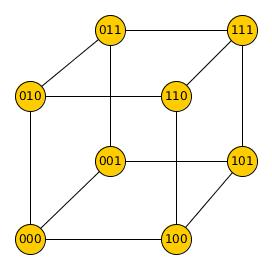
\includegraphics[scale=0.4]{graph_ape1_ex3}
    \end{flushleft}
  \end{minipage}
  \begin{minipage}{0.65\textwidth}
    \begin{flushright}
      \begin{itemize}
        \item Le graphe est $k$-régulier, car tous les nœuds sont de degré $k$.
        \item Le nombre d'arêtes est donc $|E| = \frac{2^{k} k}{2} = 12$
        \item Le graphe est biparti, car comme un seul chiffre du $k$-tuple change entre deux noeuds adjacents,
          si la somme des chiffres du $k$-tuple d'un noeud est paire, alors la somme des chiffres des $k$-tuples de ses noeuds adjacents sera impaire, et vice versa.
      \end{itemize}
    \end{flushright}
  \end{minipage}
\end{solution}

\subsection{Parcours fermés}
Formule : $\frac{(n-1)}{n}((n-1)^{k-1}+(-1)^{k})$
\begin{enumerate}
\item{Comptez le nombre de parcours fermés de longueur $k$ dans $K_{n}$ (l'ensemble des graphes complets avec $n$ nœuds)}
\item{Comptez le nombre de parcours fermés de longueur $k$ dans $K_{n,n}$ (l'ensemble des graphes bipartis avec $n$ nœuds dans chacune des partitions)}
\end{enumerate}

\begin{solution}
\begin{enumerate}
    \item \emph{TODO}
\item
	\begin{itemize}
	\item Exemple avec $n=3$ :\\
	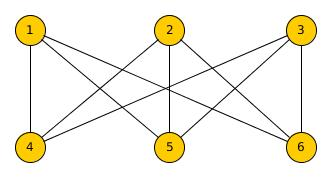
\includegraphics[width=0.4\textwidth]{graph_ape1_ex4}
	\item
	 $A = \begin{pmatrix}
	 0&0&0&1&1&1\\
	 0&0&0&1&1&1\\
	 0&0&0&1&1&1\\
	 1&1&1&0&0&0\\
	 1&1&1&0&0&0\\
	 1&1&1&0&0&0\\
	 \end{pmatrix}$

	\item $|E| = n^{2}$

	\item $A^{k} $ donne le nombre de parcours.
	\item Si $k$ est pair :
	 $A^{k} =  \left(
	 \begin{array}{c|c}
	 n^{k-1} & 0\\
	 \hline
	 0 & n^{k-1}\\
	 \end{array}
	 \right)
	 $
	\item Si $k$ est impair :
	 $A^{k} =  \left(
	 \begin{array}{c|c}
	 0 & n^{k-1}\\
	 \hline
	 n^{k-1}&0\\
	 \end{array}
	 \right)
	 $
	\item $A_{i,j}$ Le nombre de parcours de $i \rightarrow j$. Il faut prendre les valeurs où $i = j$ pour obtenir le nombre de parcours fermés
\end{itemize}
\end{enumerate}
\end{solution}

\subsection{Trouvez le nombre de parcours de longueur k du sommet A à lui-même.}
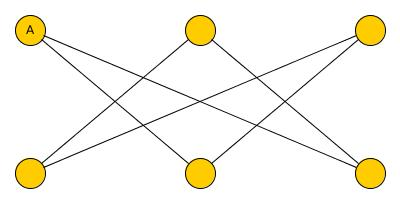
\includegraphics[scale=0.5]{graph_ape1_ex5}


\subsection{Démonstration - Les rois du graphe}
Un tournoi de $n$ joueurs est un graphe complet $K_{n}$ dans lequel on a choisi une direction pour chaque arête.
$\exists$ une arête $(u,v)$ lorsque $u$ a remporté sa partie contre $v$.
Un sommet $u$ d'un tournoi est un roi si, quel que soit le sommet $v$ du graphe,
il y a une arête $(u,v)$ où il a une arête intermédiaire $w$ et des arêtes $(u,w)$ et $(w,v)$.

Prouvez qu'il existe toujours au moins un roi.
Utiliser ce résultat pour montrer que dans le cas où aucun sommet n'a un degré entrant nul, il y a toujours au moins 2 rois.
\begin{solution}
\begin{itemize}
\item S'il n'y a pas de cycle, il suffit de remonter à l'origine pour trouver le roi.
\item S'il n'y a pas de cycle, il y a plusieurs rois.
\end{itemize}

Dans la deuxième partie, on est dans le cas d'un cycle.

Ce graphe est un exemple où il y a 3 rois.
%\includegraphics[scale=0.5]{graph_ape1_ex6}

\end{solution}
